
\chapter{Background} \label{cha:2}

Our proposed approach, V-GIM, aims to obtain the state-of-the-art performance obtained from GIM while leveraging the interpretability obtained from Variational Autoencoders (VAE). In this section, we discuss the necessary background required to understand these concepts, as they will set the basis for our own contribution.



\section{Entropy, relative entropy and mutual information}
We first discuss specific definitions from information theory. These concepts will be relevant to understand CPC and VAEs, which we discuss in a following section. The formal definitions are obtained from the book ``Elements of Information Theory" \citep{coverElementsInformationTheory2006}. The equations that contain a log function are assumed to be under base two.

\subsection{Shannon's Entropy}
Entropy measures the average amount of information required to describe a random variable \citep{coverElementsInformationTheory2006}. The entropy H(X) of a discrete random variable $X$, is formally defined as follows: 
\begin{equation}
	H(X) = -\sum_{x\in\mathcal{X}} p(x) \log p(x)  \label{eq:entropy}
\end{equation}
where $\mathcal{X}$ represents the set of events the random variable X can take, formerly known as the \textit{sample space}. Additionally, $p: \mathcal{X} \rightarrow [0, 1]$ denotes the probability density function of $X$. Hence, given an event $ x \in \mathcal{X}$, $p(x)$ corresponds to the probability of event $x$ occurring.

%[general explanation]
Assume a random variable $X$ with possible events $x_1$, $x_2$. Intuitively, when $p(x_1)$ is low, the surprise when the event $x_1$ occurs will be high. The surprise for one event is defined as follows:
%\begin{equation}
%	-p(x) \log p(x) \label{eq:surprise}
%\end{equation}
\begin{equation}
	- \log p(x) \label{eq:surprise}
\end{equation}
Hence, entropy can also be considered as the weighted average surprise over each event \citep{datasciencecoursesAliGhodsiLec2017}. 
%[algebraic explanation]
To understand why equation \ref{eq:surprise} does indeed correspond to a measure of surprise, consider an event $x \in \mathcal{X}$ with $p(x) = 1$. Note that $\log p(x) = 0$, and thus the surprise is zero. Meanwhile, if p(x) approaches $0$, $\log p(x)$ goes to $- \infty$. And hence, by the negation sign in formula \ref{eq:entropy} the surprise is large.


\begin{figure}[h]
	\centering
	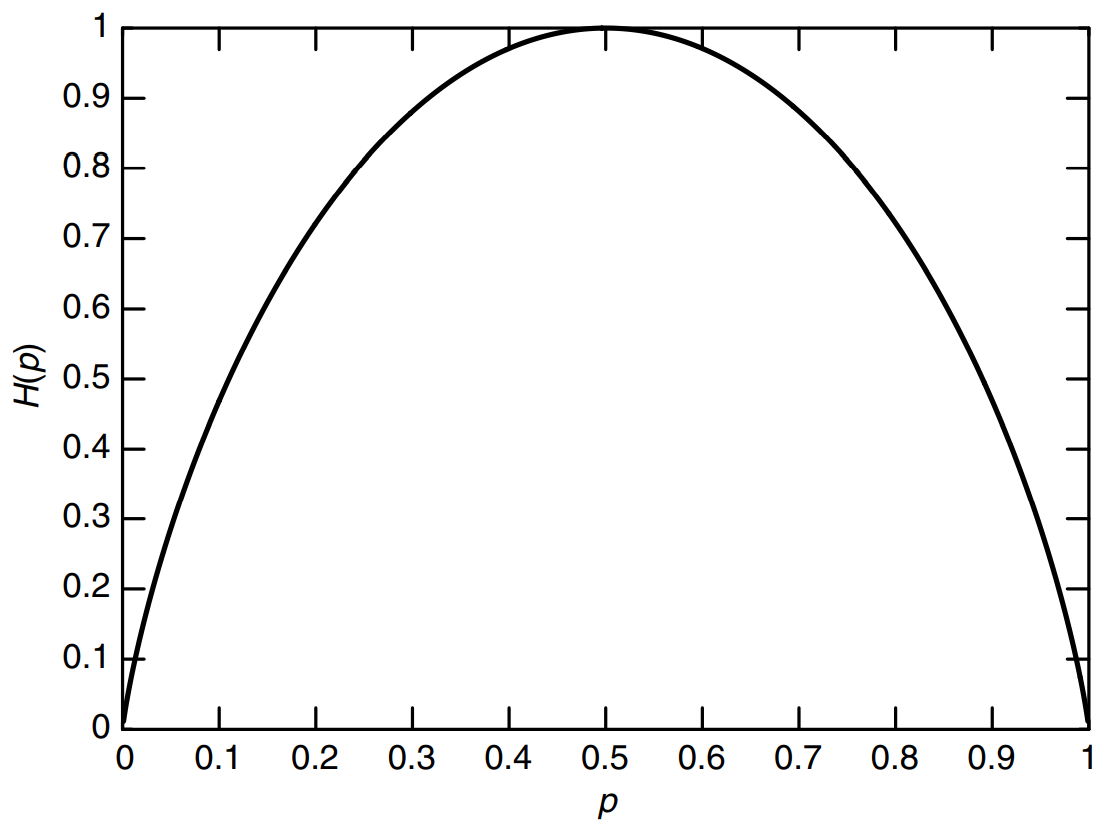
\includegraphics[width=0.4\linewidth]{screenshot005}
	\caption{$H(p)$ vs $p$ (originates from ``Elements of Information Theory", page 16)}
	\label{fig:EntropyvsP}
\end{figure}



%[book: p16: note should rename figure to axes to ” H(x) vs …”]
Figure \ref{fig:EntropyvsP} displays when entropy reaches its maximum for the case of a random variable with 2 outcomes. We can see that the entropy, and thus, the information is largest when the probability of the two outcomes is equal to each other, namely $p(x_1)=p(x_2)=0.5$. Note that for a random variable $X$ with more than two events, $H(X)$ can be larger than one.

\subsection{Relative entropy and mutual information} \label{cha:rel_entrop}
Relative entropy, also known as the Kullback Leibler (KL) divergence, is defined in equation \ref{eq:kl}, where $p$ and $q$ denote a probability density function over the same sample space $\mathcal{X}$ \citep{coverElementsInformationTheory2006}. The KL divergence quantifies the ``dissimilarity" or "divergence" between the two distributions. Note that $D(p||q)$ does not necessarily correspond to $D(q||p)$ and thus the metric is not symmetrical.

\begin{equation}
	\kl{q}{p} = \sum_{x\in\mathcal{X}}p(x) \log \frac{p(x)}{q(x)} \label{eq:kl}
\end{equation}



% was rephrased by chat gpt
The mutual information (MI) between two random variables $X$ and $Y$ can be computed as the KL divergence between their joint probability distribution, $p_{X,Y}(x,y)$, and the product of their marginal probability distributions, $p_X(x)$ and $p_Y(y)$, which is denoted as $p_X(x)p_Y(y)$ \citep{coverElementsInformationTheory2006}. The equation for mutual information then becomes:

\begin{equation}
	I(X; Y) =  \kl{p_{X, Y}(x, y)}{p_X(x) p_Y(y)}
\end{equation}

As described by Cover and Thomas in their book ``Elements of Information Theory" \citep{coverELEMENTSINFORMATIONTHEORY}, MI quantifies the amount of information $Y$ describes about $X$. An alternative definition is illustrated in \ref{eq:MI_reduce}. The equation provides us with an intuitive meaning for MI, corresponding to the surprise caused by $X$, which is reduced by the knowledge of $Y$. In sections \ref{cha:bg_reconstr} and \ref{cha:bg_nce}, we discuss how these concepts from information theory are applied in representation learning.

\begin{equation}
	I(X;Y)= H(X) - H(X|Y) \label{eq:MI_reduce}
\end{equation}



\section{Supervised machine learning and generalisation challenges}

%\textbf{TODO: purpose of section: introduce f: X -$>$ Y, but D-train is merely a subset of the data. A good f generalises well to entire D. when data is complex, many not enough labels... -> representation learning.}

% E big data set D, and training set Dtrain which trains on.

% ideas: to ensure generalisation, wants models that are as simple as possible, 
% eg vc bound: curse of dimensionality -> requires larger number of data points to ensure better generalisation.
% hence: repr learning will learn from larger dataset and generates representations for the data with smaller dimsensions. st better generalisation guarantees

We shall now discuss traditional supervised learning approaches, as these will lay the groundwork for the representation learning discussed in the following section. 

\subsection{Generalisation and curse of dimensionality}
	Consider a dataset $\D = \{ \left( \vect{x}^{(1)}, \vect{y}^{(1)} \right), \left( \vect{x}^{(2)}, \vect{y}^{(2)} \right), \dots \}$, with $\vecti{x} \in \X$ correspond to a feature vector from the feature space $\mathcal{X}$ and $\vecti{y} \in \mathcal{Y}$ its class label. Supervised machine learning problems consider the task of finding a function
	$$f: \mathcal{X} \rightarrow \mathcal{Y} \label{eq:fxy} $$
	such that given a feature vector $\vecti{x}$, a label $\vecti{y}$ can be \textit{inferred}. However, the entire dataset $\D$ is typically not available to us, and $\f$ must be derived from only a partial dataset $\Dtrain \subset \D$. A good $\f$ should not only ensure few errors on the training set $\Dtrain$, but it should also \textit{generalise} well to unseen $\vecti{x} \in \mathcal{X}$ \citep{neyshaburExploringGeneralizationDeep2017, chungUnknownExamplesMachine2019, barbieroModelingGeneralizationMachine2020}.

% towards vc dimension: smaller x results in better generalisation theories, requires smaller data
	Furthermore, when the number of dimensions of the input space $\mathcal{X}$ increases, the supervised task becomes even more challenging, requiring a larger $\Dtrain$ to ensure good generalisation. This inability of Machine Learning algorithms to manage high-dimensional data is commonly referred to as the \textit{curse of dimensionality} \citep{rustUsingRandomizationBreak1997, aremuMachineLearningApproach2020, stuartrussellArtificialIntelligenceModern2022}.
	
\subsection{Fully connected Neural Networks}
	% Deep learning	 
		Artificial Neural Networks (ANNs) address this problem of finding $\f$, by representing it as a fixed set of parameters, known as layers, which consist of a series of transformation matrices and non-linearities \citep{jainArtificialNeuralNetworks1996, kroghWhatAreArtificial2008, zhangArtificialNeuralNetwork2018}. During inference, at each layer $l$ a transformation matrix $\W^l$ is applied to the output vector from the previous layer $\vect{a}^{l-1}$. This is shown in the equation below.
		$$ \vect{z}^l = \W^l \vect{a}^{l-1} $$
		A non-linear function $\sigma: R^d \rightarrow R^d$ is then applied to $\vect{z}^{l}$, as shown in equation \ref{eq:nonlinearity}. The resulting vector $a^l$ may then again be the input for a following layer.
		$$
			\vect{a}^l = \sigma(\vect{z}^{l})	\label{eq:nonlinearity}
		$$
		
		Hence, during inference, the input vector $\vect{x}$ is propagated through each layer, resulting in a final output $\hat{y}^L$. The equation for the forward pass of a neural network with $L$ layers is described as follows: 	
		$$
			f_{\W^1 \dots \W^L}(x) = \hat{y}^L = \sigma(… \sigma( \sigma( x^T \W^1 )^T) \W^2 …)^T \W^L \label{eq:forward_pass}
		$$
		The complexity and power of a neural network are affected by the number of layers, and the choice of the number of parameters should depend on the complexity of the learning task. The architecture of a neural network, which includes the dimensions of the matrices, can be represented as a graph-like figure. An example is shown in \ref{fig:ann} where the edges between $\vect{a}^{l-1}$ and $\vect{a}^{l}$ correspond to matrix $\W^l$.

		
\begin{figure}
	\centering
	\begin{tikzpicture}[x=2.2cm,y=1.4cm]
		\message{^^JNeural network with arrows}
		\readlist\Nnod{3,4,4,2} % array of number of nodes per layer
		
		\message{^^J  Layer}
		\foreachitem \N \in \Nnod{ % loop over layers
			\edef\lay{\Ncnt} % alias of index of current layer
			\message{\lay,}
			\pgfmathsetmacro\prev{int(\Ncnt-1)} % number of previous layer
			\foreach \i [evaluate={\y=\N/2-\i; \x=\lay; \n=\nstyle;}] in {1,...,\N}{ % loop over nodes
				
				% NODES
				\node[node \n] (N\lay-\i) at (\x,\y) {$a_\i^{\prev}$};
				
				% CONNECTIONS
				\ifnum\lay>1 % connect to previous layer
					\foreach \j in {1,...,\Nnod[\prev]}{ % loop over nodes in previous layer
						\draw[connect arrow] (N\prev-\j) -- (N\lay-\i); % connect arrows directly
						%\draw[connect arrow] (N\prev-\j) -- (N\lay-\i'); % connect arrows to shifted node
					}
				\fi % else: nothing to connect first layer
			}
		}
		
		% LABELS
		\node[above=5,align=center,mygreen!60!black] at (N1-1.90) {input\\[-0.2em]layer};
	%	\node[above=2,align=center,myblue!60!black] at (N3-1.90) {hidden layers};
		\node[above=2,left=0.5cm,align=center,myblue!60!black] at (N3-1.90) {hidden\\[-0.2em]layers};
		\node[above=8,align=center,myred!60!black] at (N\Nnodlen-1.90) {output\\[-0.2em]layer};
		
		
	\end{tikzpicture}
	\caption{Visual representation of a neural network}
	\label{fig:ann}

\end{figure}




%\begin{tikzpicture}[x=2.7cm,y=1.6cm]
%	\message{^^JNeural network activation}
%	\def\NI{5} % number of nodes in input layers
%	\def\NO{4} % number of nodes in output layers
%	\def\yshift{0.4} % shift last node for dots
%	
%	% INPUT LAYER
%	\foreach \i [evaluate={\c=int(\i==\NI); \y=\NI/2-\i-\c*\yshift; \index=(\i<\NI?int(\i):"n");}]
%	in {1,...,\NI}{ % loop over nodes
%		\node[node in,outer sep=0.6] (NI-\i) at (0,\y) {$a_{\index}^{(0)}$};
%	}
%	
%	% OUTPUT LAYER
%	\foreach \i [evaluate={\c=int(\i==\NO); \y=\NO/2-\i-\c*\yshift; \index=(\i<\NO?int(\i):"m");}]
%	in {\NO,...,1}{ % loop over nodes
%		\ifnum\i=1 % high-lighted node
%			\node[node hidden]
%			(NO-\i) at (1,\y) {$a_{\index}^{(1)}$};
%			\foreach \j [evaluate={\index=(\j<\NI?int(\j):"n");}] in {1,...,\NI}{ % loop over nodes in previous layer
%				\draw[connect,white,line width=1.2] (NI-\j) -- (NO-\i);
%				\draw[connect] (NI-\j) -- (NO-\i)
%				node[pos=0.50] {\contour{white}{$w_{1,\index}$}};
%			}
%		\else % other light-colored nodes
%			\node[node,blue!20!black!80,draw=myblue!20,fill=myblue!5]
%			(NO-\i) at (1,\y) {$a_{\index}^{(1)}$};
%			\foreach \j in {1,...,\NI}{ % loop over nodes in previous layer
%				%\draw[connect,white,line width=1.2] (NI-\j) -- (NO-\i);
%				\draw[connect,myblue!20] (NI-\j) -- (NO-\i);
%			}
%		\fi
%	}
%	
%
%	
%
%	
%\end{tikzpicture}




	
	% [cost function, gradient descent, backpropagation]
		During training the ANN's parameters $\W = \{\W^1$ \dots $\W^L\}$, are optimised according to the learning problem. The viability of the parameters is quantified by the loss function $\mathcal{L}$ over a batch of $n$ training samples, shown as follows:
		$$
			\mathcal{L}(\W) = \frac{1}{n}\sum_{i=1}^n e(\vecti{y}, \vecti{\hat{y}}) \label{eq:generic_loss}
		$$
		where $\vecti{y}$ corresponds to the ground truth label and $\vecti{\hat{y}} = f_{\W}(\vecti{x})$. The error function $e(\cdot)$ can be chosen depending on the task, for instance by mean squared error for regression or cross entropy for classification problems.
		
		The parameters $\W^1 \dots \W^L$ are typically achieved through iterative minimisation of the loss function. This is achieved using backpropagation, an efficient algorithm which computes the partial derivates with respect to each parameter $\W^l_{ij}$. Updating the parameters in the opposite direction of the partial derivative allows for an iterative estimation of a local minimum, which is demonstrated in the following equation using stochastic gradient descent:
		$$
			\W^l_{ij} \leftarrow \W^l_{ij} - \alpha \frac{\partial \mathcal{L}}{\partial \W^l_{ij}}
		$$
		The details of computing the partial derivatives using backpropagation are beyond the scope of this thesis.
		% TODO: kan anders omshcijrven: "while the details of... are not important for our contributions in this thesis, it is important to recognise that a good choice for the loss function is important, as this will decide on meaningful learning

	
	\subsection{Towards lower dimensional feature spaces}
	
	Supervised learning through ANNs is often successful, even when dealing with complex problems. However, achieving high performance on the training set does not guarantee good generalisation to new data. As problems become more complex, the use of larger amounts of labelled data is required to ensure good generalisation. For complex feature vectors, a more sophisticated architecture may be necessary, which in turn requires even more data to prevent overfitting. % TODO: MAYBE I NEED A REFERENCE?
	
	In cases where labelled data is scarce, ANNs may appear to perform well on the training set, but their generalisation performance to data outside the training set can be poor. The performance of ANNs is thus heavily dependent on the choice of data representation \citep{bengioRepresentationLearningReview2013}. As a consequence, a lot of effort in the machine learning pipeline is invested in feature engineering \citep{zhengFeatureEngineeringMachine2018}, which involves extracting useful features from the feature space $\mathcal{X}$, removing redundant information, and reducing the dimensionality of the feature space \citep{valiDeepLearningLand2020} to obtain a good representation $\vect{z} \in \mathcal{Z}$ that is easier to work with. Rather than learning the mapping function directly on the data, $\vect{x} \in \mathcal{X}$ is first transformed into a lower-dimensional representation $\vect{z} \in \mathcal{Z}$. The mapping function from equation \ref{eq:fxy} is now:
	$$f: \mathcal{Z} \rightarrow \mathcal{Y} \label{eq:fxz} $$
	
	However, feature engineering is a time-consuming and often manual process that requires domain knowledge and expertise \citep{przybyszewskiUseDomainKnowledge2017, weiIntegrationDomainKnowledgeGuided2021}. In the following section we discuss how part of the manual labour of finding good representations from data can be relieved with unsupervised learning approaches, which automate this process. These representations could then be used as the input for a supervised predictor $\f$ or \textit{downstream task} \citep{zhangOmiEmbedUnifiedMultiTask2021}.


\section{Representation learning through reconstruction error} \label{cha:bg_reconstr}

% TODO: OPMERKING BART: WAT IS HET VERSCHIL TUSSEN REPRESENTATIE EN LATENT REPR?

% while supervised learning learning finds f given x -> y. performance gains may be obtained by manually transformating T(x) = z s.t f(z) = y. Self supervised representation learning attempts to automate the process of finding T.

%[what is repr learning]
One of the challenges in supervised learning is the constant need of large amounts of labelled data $\Dtrain = \{ \left( \vect{x}^{(1)}, \vect{y}^{(1)} \right), \left( \vect{x}^{(2)}, \vect{y}^{(2)} \right), \dots \}$. When this set is scarce, or the task becomes too complex to ensure good generalisation, transforming the feature space $\X$ to a lower-dimensional space $\Z$ can be a good solution to aid with learning for the downstream task $\f$. Meanwhile, an abundant amount of unlabelled data may already exist. Hence, when a labelled dataset is small, we would like to leverage a larger unlabelled dataset as basis for learning.

In this section we investigate two self-supervised learning paradigms which learn the following transformation function solely from a feature space $\X$ and thus do not require any labels:
$$T: \X \rightarrow \Z$$
such that the simplified representations obtained from $\T$ can serve as the input for a downstream task as follows:
\begin{align*}
	T(\vect{x}) &=  \vect{z} \\
	f(\vect{z}) &= \vect{y} 
\end{align*}
This process of learning a mapping function $\T$ which translates a feature vector $\vect{x}$ to a lower-dimensional representation $\vect{z}$ is commonly referred to as representation learning \citep{le-khacContrastiveRepresentationLearning2020}. 

In the following two subsections we discuss two paradigms of representation learning with ANNs. The first paradigm learns representations by minimising a reconstruction error. The second learns its representations by contrasting them against noise. These two paradigms will lay the basis for our own contributions in chapter three.

\subsection{Autoencoders}
The encoding problem, introduced by Ackley and Hinton in 1985 \citep{ackleyLearningAlgorithmBoltzmann1985}, and later referred to as the autoencoder by Rumelhart et al. in 1986 \citep{rumelhartLearningInternalRepresentations1988}, considers the problem of learning compressed representations through neural networks \citep{rumelhartLearningInternalRepresentations1988, bankAutoencoders2021}. This is achieved through an ANN architecture consisting of two functions, an \textit{encoder} $E(\vect{x}) = \vect{z}$ and a \textit{decoder} $D(\vect{z}) = \vect{\tilde{x}}$.
%The first block is the encoder $E$ and receives input data which it encodes into a lower dimensional representation. The second block, called the decoder $D$, receives as input the latent representation and is tasked to reconstruct the original input. 
The lower-dimensional \textit{encoding} $\z$ obtained from $E(\x)$ will then serve as representation for downstream task $\f$.
The functions $\E$ and $D(\cdot)$ are simultaneously optimised by minimising the reconstruction error shown in the following equation:
\begin{equation}
	\mathcal{L} = \sum_{i = 1}^N l(\vecti{x}, \vecti{\tilde{x}})
\end{equation}
where $l$ refers to the error for a single data point, for instance the $l^2$-norm and $N$ the number data points. The dimension of $\vect{z}$ is typically smaller than the original dimension of $\vect{x}$. This results in the encoder having to define encodings that are as ``informative" as possible to reconstruct the original data \citep{bankAutoencoders2021}.

An example autoencoder architecture is depicted in figure \ref{fig:autoencoder}. Since an autoencoder is in fact a single ANN and $\z$ corresponds to the output produced by an intermediate hidden layer, $\z$ is also commonly referred to as a \textit{latent} representation. The space of all latent representations $\Z$ is known as the \textit{latent} space.
	\begin{figure}
		\centering
		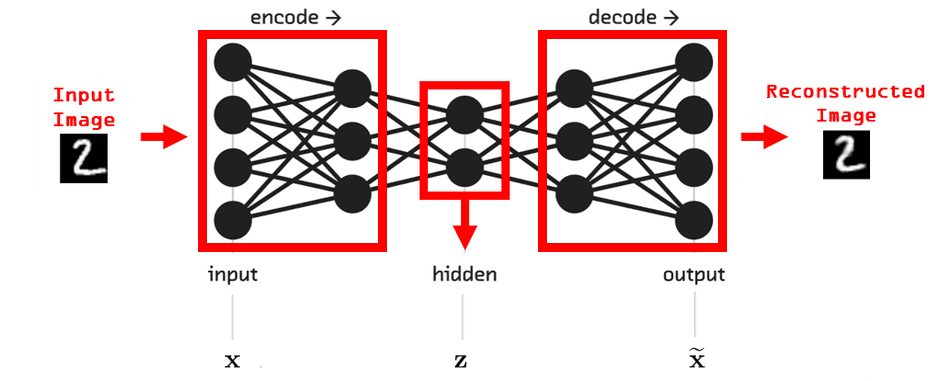
\includegraphics[width=0.7\linewidth]{autoencoder}
		\caption{Autoencoder architecture, adapted from \citep{karagiannakosHowGenerateImages2018}.}
		\label{fig:autoencoder}
	\end{figure}
While capable of learning compressed representations, autoencoders do not pose any restrictions on the latent space $\Z$. As a result, the representations may be meaningful to computers, but non-interpretable to humans. For instance, given the left image depicted in figure \ref{fig:latent_space_2d} which depicts an autoencoder's two dimensional latent space, it is almost impossible to infer in advance what the corresponding digit would be when interpolating a new $\z$ somewhere in between the encodings corresponding to digit 0 (red) and 1 (blue). In addition, slight changes to $\z$ may result in significant changes to its decoded counterpart $\x$. Finally, attempting to understand an autoencoders latent space $\Z$ becomes even more infeasible as the dimension of $\Z$ increases.

\begin{figure}
	\centering
	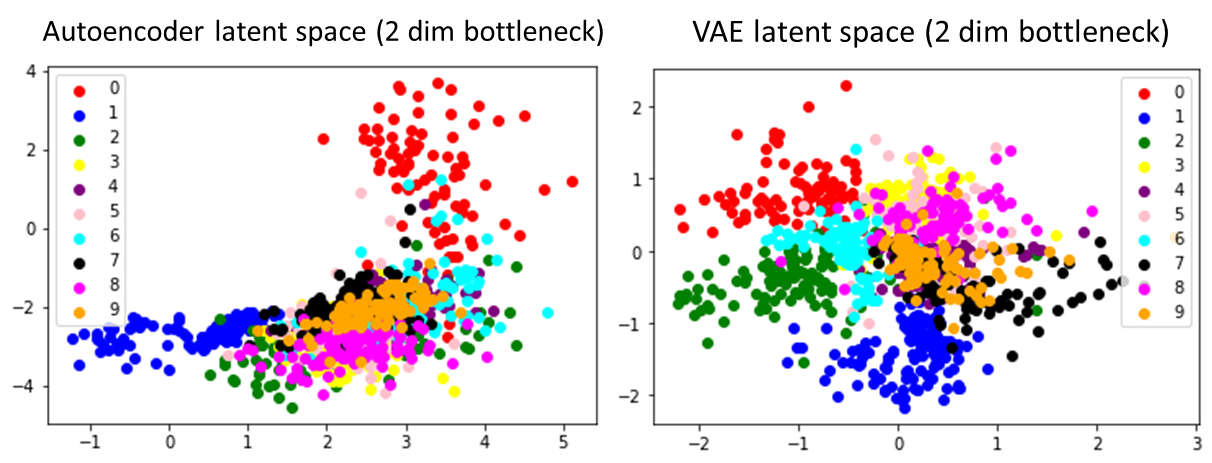
\includegraphics[width=0.7\linewidth]{screenshot021}
	\caption{ Latent space of autoencoder (left) and VAE (right), learned from the MNIST dataset \citep{lecunGradientbasedLearningApplied1998}, a dataset consisting of images of handwritten digits between 0 and 9. The ANNs have not received any explicit information of the labels of the dataset. 
	%The VAE's latent space, depicted in the right image, is optimised to be standard normally distributed. The latent vectors $\vect{z}$ are distributed according to the two-dimensional normal distribution $\sample{\vect{z}}{\standardnormal}$, where $\bm{\mu}$ is the two dimensional zero vector. $\identitymtx$ is the $2 \times 2$ covariance matrix with ones on the diagonal and zeroes elsewhere.
}
	\label{fig:latent_space_2d}
\end{figure}



\subsection{Variational autoencoders}
% notes: 
%1) discuss why, (latent space gaussian)
%2) architecture predicting values
%3) explicit elbo (where q is optimised to be Gaussian) and give intuitions how it squishes all data points together
%4) can be used for latent space, or also 
%4) link with maximising likelihood -> p(x) and how minimises kl divergence between approx and kl divergence

Similar to traditional autoencoders, variational autoencoders (VAE) learn representations that contain the important information necessary to reconstruct the data. VAEs maintain the same structure from autoencoders, consisting of encoder $E(\vect{x}) = \vect{z}$ and decoder $D(\vect{z}) = \vect{\tilde{x}}$. However, an additional constraint is applied to the latent space $\Z$ \citep{doerschTutorialVariationalAutoencoders2021, davidfosterVariationalAutoencoders2023, kingmaAutoEncodingVariationalBayes2022, kingmaIntroductionVariationalAutoencoders2019, cinelliVariationalMethodsMachine2021}. In fact, the latent representations $E(\vect{x}) = \vect{z}$ are samples from multivariate distributions, which we will denote by 
$$\sample{\vect{z}}{\qvae}$$
Thus, given a feature vector $\x$, we obtain its corresponding encoding or latent representation $\z$ by taking a sample from a distribution. We will define $q$ in more detail in a following paragraph. The encoder function $\E$ in VAEs is thus nondeterministic and computing $E(\vect{x}) = \vect{z}$ twice may result in two different $\z$s both corresponding to the same $\x$. In a following paragraph we will discuss how to achieve this nondeterministic behaviour using ANNs.

By defining the latent representations as samples from distributions, we can pose the same constraints on the quality of the representations $\z \in \Z$ as in traditional autoencoders, but also additional constraints on how the latent space $\Z$ is organised. The additional constraints posed by VAEs on $\Z$ will result in a more interpretable space, where $\z$'s underlying components can be better understood. This will be achieved by enforcing each distribution $\qvaeEmptyZandXI$ corresponding to a particular $\vecti{x}$, to be ``similar" to a chosen prior distribution $p(\z)$. Typically, the prior $p(\z)$ is set to the standard normal distribution $\standardnormal$ \citep{davidfosterVariationalAutoencoders2023}. The result of this setup can be observed in the latent space depicted in the right plot of figure \ref{fig:latent_space_2d} where all $\z$s are attracted to the origin.

In the following subsections, we will explore VAEs in more detail. We begin with a discussion on the process of imposing constraints on $\Z$, which leads to the VAE loss function. Next, we investigate how ANNs can be utilised to simulate sampling from distributions. Finally, we examine how VAEs enable the creation of interpretable representations and how they can be used to generate novel data.




\subsubsection{The loss function}	
% def q

	So far, we have learned that Variational Autoencoders (VAEs) use an encoder $E(\x) = \z$ to create a latent representation $\z$ of the input feature vector $\x$, where $\z$ is a sample from the distribution $\sample{\z}{\qvae}$. Equivalently, for each $\x$, there exists a unique distribution $q(\z)$ that characterizes $\qvae$ \citep{volodymyrkuleshovVariationalAutoencoder2023}. We can then define $\qvae$ as a Gaussian with independent components, parametrised by $\mufat$ and covariance matrix $\diagsigma$. We obtain the the following definition:
	\begin{equation}
		\qvae = \normalNoI \label{eq:definition_q}
	\end{equation}
	where $\diagsigma$ denotes the covariance matrix with $\sigmafat$ on the diagonal and zeroes elsewhere. It is important to recognise that $\mufat$ and $\sigmafat$ are different for every $\x$. The two parameters will be computed by an ANN.


% loss
	The representations are optimised to minimise two measurements: one, the reconstruction error, and secondly, the dissimilarity from the latent distributions to a chosen prior $p(\z)$. %$\standardnormal$.
	The loss function to be optimised for a single data point $\vecti{x}$ is shown in the equation below.
	\begin{equation}
		\mathcal{L} (\vecti{x}) = \elboexplicit \label{eq:elbo_explicit_intial}
		%\mathcal{L}_{\theta, \phi} (\vecti{x}) = \elboexplicit \label{eq:elbo_explicit_intial}
	\end{equation} % src: ref to slides ugent
	Here, $p(\cdot)$ refers to the prior distribution, which is different from $\pthetaxzi$.
	% 1) reconstruction error
	Although $\mathcal{L}$ may seem daunting at first, we will decompose its components. The loss function is made up of two terms, the left term corresponds to the reconstruction error, while the second term poses constraints on the latent space. Let us focus on the reconstruction term first.
	
	\begin{equation}
		\reconstr \label{eq:reconstr}	
	\end{equation}

	In a traditional autoencoder we optimise $D(E(\vecti{x})) = \vecti{\tilde{x}}$ such that $\vecti{x} \approx \vecti{\tilde{x}}$. We will now show that the reconstruction term in equation \ref{eq:reconstr} achieves a similar goal for VAEs. Here, $\pthetaxzi$ is a distribution over $\vecti{z}$ where $\vecti{x}$ is a constant, and the latent representation $E(\vecti{x}) = \vecti{z}$ is sampled from the Gaussian distribution $\sample{\vecti{z}}{\qphizxblank}$. The objective is to ensure that $D(\vecti{z}) \approx \vecti{x}$. However, since $\vecti{z}$ is sampled from a Gaussian distribution, the $\vecti{z}$'s close to the mean $\mui$ are more likely to be sampled than those further away. Thus, for these $\vecti{z}$'s, we'd like the probability of corresponding to the actual $\vecti{x}$ to be high, or equivalently we want $\pthetaxzi \approx 1$ \citep{cinelliVariationalMethodsMachine2021}. Finally, by adding a negative sign in front, maximising this probability is equivalent to minimising the negative probability. In practice this term is approximated through mini-batches with the mean squared error. %todo: look into max like estim, as there hopefully i can find a meaningful defintion for "maximising..."
	

% 2) latent space
	Optimising the second term of equation \ref{eq:elbo_explicit_intial} poses the constraints on the distributions $\qphizxblank$. 
	\begin{equation}
		%\latentspaceconstraintstandardgaussian
		\latentspaceconstraint \label{eq:latent_space_constraint}		
	\end{equation}
	Again, this metric should be minimised. As we discussed in chapter \ref{cha:rel_entrop}, KL divergence can be considered as a dissimilarity measure between two distributions. Hence, this value is small when the two distributions are similar. The prior distribution $\pzblank$ is a fixed distribution which is chosen by the user, typically defined as $\standardnormal$. Minimising this metric will result in moving each distribution $\qphizx$, corresponding to a value $\vecti{x}$, close to $\standardnormal$. This idea is depicted in figure \ref{fig:twogaussiandistributions}. When $\pzblank = \standardnormal$, equation \ref{eq:latent_space_constraint} becomes:
	$$\latentspaceconstraintstandardgaussian$$
	
	\begin{figure}
		\centering
		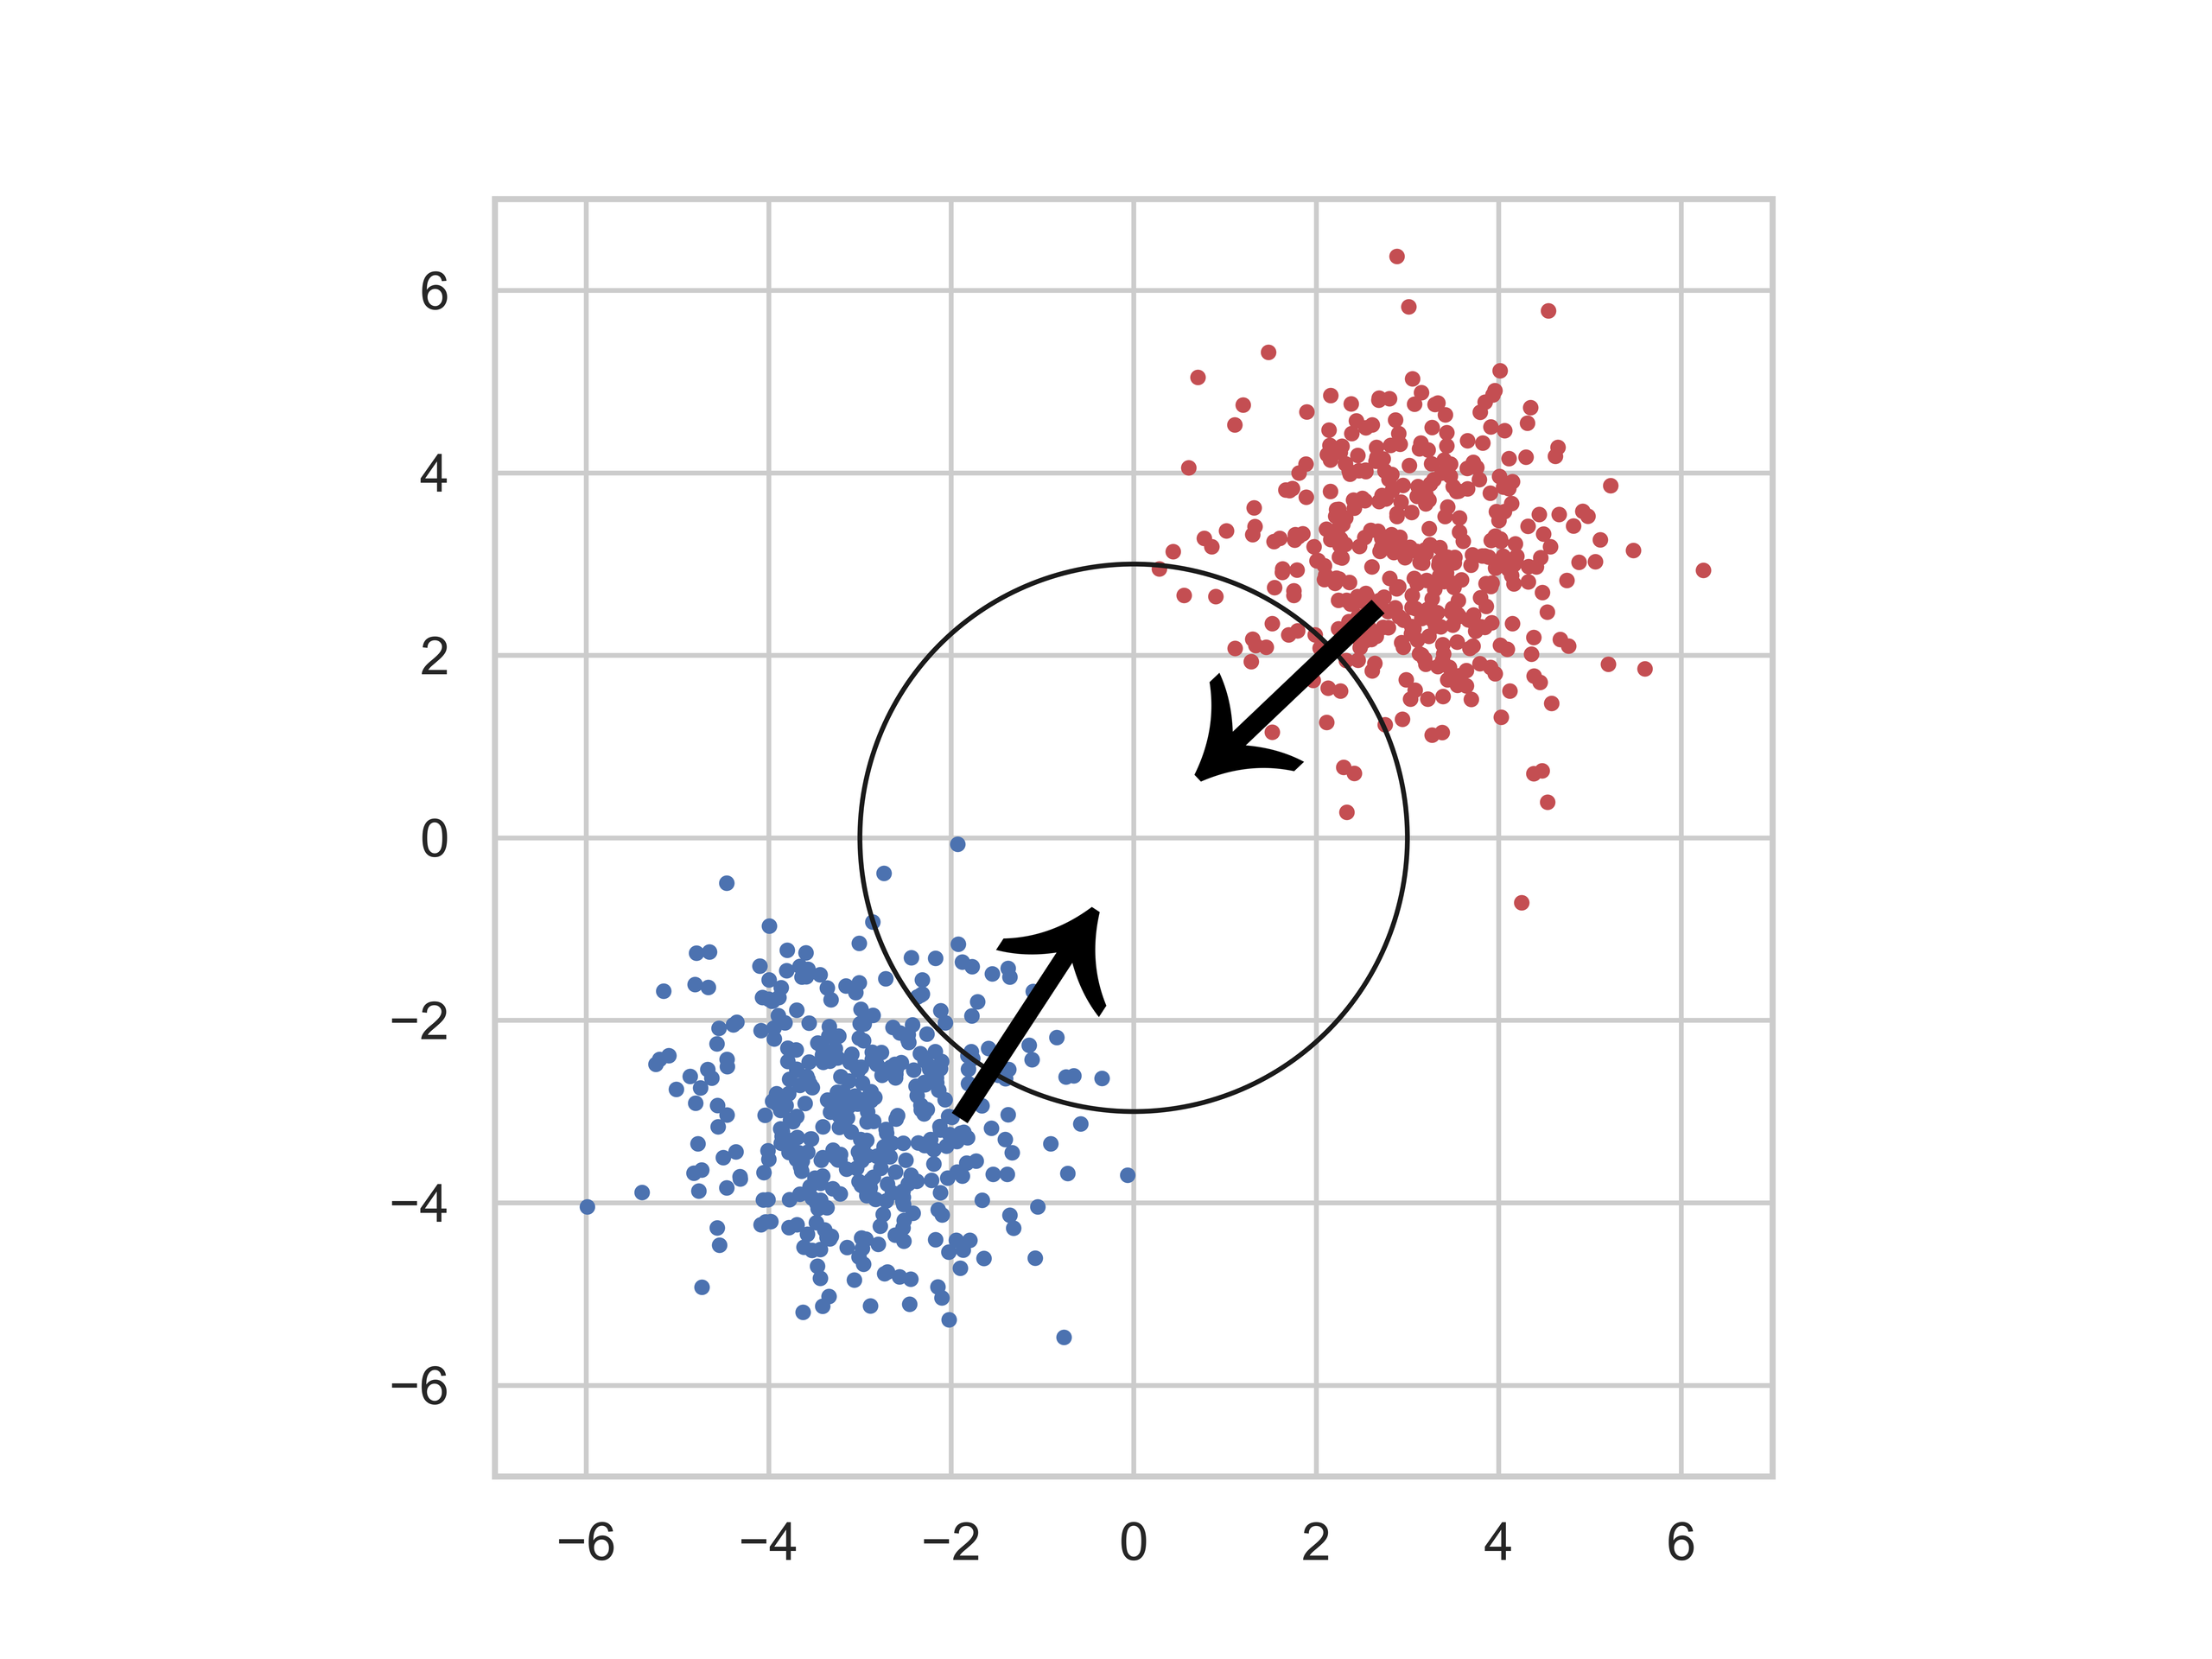
\includegraphics[width=0.7\linewidth]{two_gaussian_distributions}
		\caption{200 samples $\vecti{z}$ and $\vectj{z}$ from feature vectors $\vecti{x}$ and $\vectj{x}$, respectively, represented by red and blue data points. The prior $p(\vect{z})$ is set to the standard normal, and the regularisation term of VAE's loss pushes the latent space towards the origin.}
		\label{fig:twogaussiandistributions}
	\end{figure}
	When $\qphizxblank = \normal$, one can algebraically prove, that optimising the above equation is equivalent to optimising the following \citep{kingmaAutoEncodingVariationalBayes2022}: 
	\begin{equation}	
		\kl{\normal}{\standardnormal} = \latentspaceconstraintclosedform
	\end{equation}
	where $\sigma_k^{(i)}$ and $\mu_k^{(i)}$ correspond to the components of the predicted vectors $\sigmai$ and $\mui$, respectively. The latent space has dimensionality $D$.
	



%\textbf{How: predict distributions}

\subsubsection{Simulating distributions through neural networks}
	Computing $E(\xith)$ results in encoding $\zith$ which is sampled from $\sample{\zith}{\qvaeEmptyZandXI}$. We will now discuss how ANNs can emulate the stochastic behaviour of sampling from a distribution. As discussed in equation \ref{eq:definition_q}, distribution $\qvaeEmptyZandXI$ is parametrised as a Gaussian with mean $\mui$ and covariance matrix $\diagsigmai$. The entire distribution can thus be modelled by an ANN which takes as input $\xith$ and generates the two corresponding vectors $\mui$ and $\sigmai$. Finally, a sample $\vecti{z}$ can be obtained as follows:
	\begin{equation}
		\vecti{z} = \mui + \sigmai \odot \epiloni
	\end{equation}
	where $\epiloni$ corresponds to a sampled value $\samplestandardnormal{\epiloni}$ and $\odot$ is element-wise multiplication. Computing $\vecti{z}$ through $\epiloni$, rather than directly sampling from $\sample{\vecti{z}}{\normal}$ is referred to as the parametrisation trick and allows for gradients to freely backpropagate through the layer \citep{davidfosterVariationalAutoencoders2023}. The decoder $D(\zith) = \vecti{\tilde{x}}$ can remain identical to the traditional autoencoder's decoder. An overview is presented in figure \ref{fig:vae-repr}.
	
	\begin{figure}[h]
	\centering
	\tikzstyle{arrow} = [thick,->,>=stealth]
	\begin{tikzpicture}[
		AnnNode/.style={trapezium, draw=black,
			trapezium stretches=true,
			minimum width=2cm, 
			minimum height=1.5cm,
			rotate=-90,
			trapezium angle=75,
			very thick},
		]
		
		\node[AnnNode] (enc) {\rotatebox{90}{$E(\xith)$}};
		\node[AnnNode] (dec) [right of=enc, xshift=1.5cm] {\rotatebox{90}{$D(\zith)$}};
		
		% enc edges
		\draw[->] ++(-2.5, 0) -- (enc.south) node[above, midway] {$\xith \in \D$};
		\draw[->] 
		[transform canvas={yshift=.7em}] 
		(enc.north) -- ++(1.5, 0) node[above, midway] {$\mui$};
		\draw[->] 
		[transform canvas={yshift=-.7em}] 
		(enc.north) --  ++(1.5, 0) node[below, midway] {$\sigmai$};
		
		\node 
		[transform canvas={xshift=5.5em}] 
		(bracket1) at (enc.north) {\Huge \} };
		
		\node 
		[transform canvas={xshift=10em}] 
		(sample z) at (enc.north) {$\sample{\zith}{\qvaeEmptyZandXI}$ };
		
		
		
		% dec edges
		\draw[->] ++(-2.5, -2.5) -- (dec.south) node[above, midway] {$\zith$};
		\draw[->] 
		(dec.north) -- ++(1.5, 0) node[above, midway] {$\vecti{\tilde{x}}$};	  		
		
		
		
	\end{tikzpicture}
	\caption{High level view of a VAE.}
	\label{fig:vae-repr}
\end{figure}





% from img
% Both blocks depict a neural network. The upper block is the encoder and the lower block the decoder. The upper block receives a data points $\vect{x}$ and produces the parameters of $\qphizx$. Since we choose to model $\qphizx$ as a Gaussian with independent components, the covariance matrix $\covariancemtx$ is zero everywhere except for the diagonal. This way the diagonal values, representing the standard deviations, can be represented via a single vector $\sigmai$. The vectors $\mui$ and $\sigmai$ are $\mu(\vecti{x})$ and $\sigma(\vecti{x})$, respectively. These are the output of the encoder block and form the parameters for $\qphizx$. A single neural network with parameter weights $\phi$ is used to simulate $\qphizx$ for every $\vecti{x} \in \mathcal{D} $. This strategy of sharing $\phi$ across data points is refered to as "amortised variational inference" \cite{kingmaIntroductionVariationalAutoencoders2019}.
	
	
	
	




	
	


\subsubsection{Generating new data and interpretability}	
	Due to the VAE's regularisation term all encodings are pushed towards the centre as depicted in figure \ref{fig:twogaussiandistributions}. Additionally, the space of encodings corresponding to a single $\xith$ is an entire neighbourhood around a particular $\mufat$ and $\sigmafat$. These two properties ensure a well covered and uninterrupted space around the origin with smooth transitions on the generative factors between latent representations \citep{davidfosterVariationalAutoencoders2023}. As a result, new samples from the dataset can be generated by discarding the VAE's encoder and providing standard normal noise to the decoder instead. It is important to understand that this method only works for VAEs and not for the traditional autoencoder. This is because autoencoders do not pose any additional constraints on the latent space. Generating new data points from random noise via a traditional autoencoder may result in nonsense generations as the random noise may be too different from the latent space it was trained on. As a result, there are no guarantees that the autoencoder's decoder will generalise to these random representations.
	
	Additionally, for the same reason, we can interpolate between encodings obtained from the data. The interpolated encoding can then decoded to the original space. We can observe the specific information contained in each of the representations' features through the decoder, resulting in a significant improvement in interpretability.
	% TODO: if time permits, this sectino could be written better ^^ ik zou met ven diagrammen kunnen werken.
	
	% TODO: maybe check if everything is present and argumentation is okay.	
	%	o reiley:
		%Firstly, we now have a well-defined distribution that we can use for choosing points in the latent space—the standard normal distribution. Secondly, since this term tries to force all encoded distributions toward the standard normal distribution, there is less chance that large gaps will form between point clusters. Instead, the encoder will try to use the space around the origin symmetrically and efficiently.
		
		
		%\textit{Previously, we saw how there was no requirement for the latent space to be continuous—even if the point (–2, 2) decodes to a well-formed image of a sandal, there was no requirement for (–2.1, 2.1) to look similar. Now, since we are sampling a random point from an area around $z_mean$, the decoder must ensure that all points in the same neighborhood produce very similar images when decoded, so that the reconstruction loss remains small. This is a very nice property that ensures that even when we choose a point in the latent space that has never been seen by the decoder, it is likely to decode to an image that is well formed.} - o reiliy
		%
		
	
	
	
	
	
	
	
	
	



%\subsubsection{[TODO] Relation with variational inference / derivation of ELBO loss}
%	
%	%A mapping function $f_W(x) = y$ can be predict distributions by predicting the parameters of the the distribution (mu, sigma for Gaussian distributions).
%	%
%	%Rather than directly learning parameters $\phi$ that map a data point $\vecti{x}$ to latent distribution $p(\vect{z} \mid \mathbf{x}^{(i)})$, an \textit{approximate distribution} $\qzx$ is learned that approximates $p(\vect{z} \mid \vecti{x})$. Through gradient descent parameters for $\phi$ can be achieved, by minimising the KL divergence between the two distributions. $\condq{\vect{z}}{\vecti{x}}$ will is expressed as Gaussian distribution.
%	%
%	%
%	%\begin{equation}
%	%	\kl{\qprobzx}{\probzx} \label{eq:kl_q_p}
%	%\end{equation}
%	%
%	%Yet, the idea is nice, optimising $\qprobzx$ to approximate $\probzx$ sounds nice, it is only possible when $\probzx$ is known, which it is not. If it was, there was no need to approximate it.
%	%
%	%Equation \ref{eq:kl_q_p} is thus intractable to compute, yet the following is true:
%	%
%	%\begin{equation}
%	%	\begin{aligned}
%	%		\kl{\qprobzx}{\probzx} & = \expectedsamplezq \left[ \log \frac{\qzx}{\pzx} \right] \\
%	%		& = ... (todo) \\
%	%		& = - \left( \elbo \right) + \logevidence
%	%	\end{aligned}
%	%\end{equation}
%	%
%	%By replacing the terms, we obtain the following equation:
%	%
%	%\begin{equation}
%	%	\begin{aligned}
%	%		\logevidence & = 
%	%		\klapproxposterior + \elbo \\
%	%		& = \klapproxposterior  + \lelbo
%	%	\end{aligned}
%	%\end{equation}
%	%
%	%We can observe that the KL divergence between the true and approximate posteriors, $p$ and $q$ respectively, is bounded by $\logevidence$. Hence, although $\pzx$ is unknown, maximising $\lelbo$ results in minimising the KL divergence. Also notice that $\kl{\qprobzx}{\probzx} >= 0$, and thus the maximum value for $\lelbo$ results in a KL divergence between the posteriors of zero. It thus suffices to maximise $\lelbo$, or equivalently minimise $-\lelbo$. The loss for a single data point $\vecti{x}$ then becomes
%	
%	%TODO \textbf{todo: in paper variational bayes, they refer to p(x) as p theta, but in slides ugent not?}. \textbf{todo: why cant p(x) be very big then? probably has something to do with jensens inequality.}
%	
%	
%	
%	
%	\begin{equation}
%		\begin{aligned}
%			- \lelbo & = - \elbo \\  
%			& = \elboexplicit \label{eq:elboexplicit} \\
%		\end{aligned}	
%	\end{equation} % src: ref to slides ugent
%	
%	Where the first term is reconstruction error and second is regularisation. Hence minimising the KL divergence between the two posteriors is equivalent to minimising the divergence between the approximate posterior $\qzx$ and the \textbf{marginal or prior?} $\pz$.
%	
%	$p(z)$ in the equation is usually chosen to be the standard normal distribution $\mathcal{N}(0, I)$, such that a closed form solution exists. As such, when $p(z)$ corresponds to the standard normal, and $\qzx$ is a multidimensional Gaussian with mean vector $\mui$ and covariance matrix with independent dimensions, such that the diagonal corresponds of a vector standard devisations $\sigmai$, then the KL divergence has the following closed form:
%	
%	\begin{equation}	
%		\kl{\normal}{\standardnormal} = \latentspaceconstraintclosedform
%	\end{equation}
%	
%	For the equation above, gradients can easily be back propagated through machine learning libraries such as Tensor Flow. We still require a method for computing the gradient of the first term in $\lelbo$. % todo: gradient van linker kan door sampling en mini batch.
%	
%	
%	
%	
	
	
	
	
	
	
	
	%Recent Advances in Autoencoder-Based:
	%Representation Learning https://arxiv.org/pdf/1812.05069.pdf
	%they speak about disentanglement of vae and indepndent features
	
	%Understanding disentangling in β-VAE
	%https://arxiv.org/pdf/1804.03599.pdf
	%"β-VAE aligns latent dimensions with components that make different contributions to reconstruction"
	%Our key hypothesis is that β-VAE finds latent components which make different contributions to the log-likelihood term of the cost function (Eq. 5). These latent components tend to correspond to features in the data that are intuitively qualitatively different, and therefore may align with the generative factors in the data.
	
	
	
	
	
	
	
	
	
	
	
	%- \subsubsection{reparametrisation trick}
	%o reiley:
	%\textit{THE REPARAMETERIZATION TRICK
	%	Rather than sample directly from a normal distribution with parameters $z_mean$ and $z_log_var$, we instead sample epsilon from a standard normal and then manually adjust the sample to have the correct mean and variance.}
	%\textit{This is known as the reparameterization trick and is important as it means gradients can backpropagate freely through the layer. By keeping all of the randomness of the layer contained within the variable epsilon, the partial derivative of the layer output with respect to its input can be shown to be deterministic (i.e. independent of the random epsilon), which is essential for backpropagation through the layer to be possible.}
	
	%\subsubsection{the loss function - from oreiley}
	%The Loss Function
	%Previously, our loss function only consisted of the reconstruction loss between images and their attempted copy after being passed through the encoder and decoder. The reconstruction loss also appears in a variational autoencoder, but we require one extra component: the Kullback–Leibler (KL) divergence term.
	%
	%KL divergence is a way of measuring how much one probability distribution differs from another. In a VAE, we want to measure how much our normal distribution with parameters z_mean and z_log_var differs from a standard normal distribution. In this special case, it can be shown that the KL divergence has the following closed form:
	%
	%kl_loss = -0.5 * sum(1 + z_log_var - z_mean ^ 2 - exp(z_log_var))
	%or in mathematical notation:
	%
	%The sum is taken over all the dimensions in the latent space. kl_loss is minimized to 0 when z_mean = 0 and z_log_var = 0 for all dimensions. As these two terms start to differ from 0, kl_loss increases.
	%
	%In summary, the KL divergence term penalizes the network for encoding observations to z_mean and z_log_var variables that differ significantly from the parameters of a standard normal distribution, namely z_mean = 0 and z_log_var = 0.
	%
	%Why does this addition to the loss function help?
	%
	%Firstly, we now have a well-defined distribution that we can use for choosing points in the latent space—the standard normal distribution. Secondly, since this term tries to force all encoded distributions toward the standard normal distribution, there is less chance that large gaps will form between point clusters. Instead, the encoder will try to use the space around the origin symmetrically and efficiently.
	%
	%In the original VAE paper, the loss function for a VAE was simply the addition of the reconstruction loss and the KL divergence loss term. A variant on this (the 
	%-VAE) includes a factor that weights the KL divergence to ensure that it is well balanced with the reconstruction loss. If we weight the reconstruction loss too heavily, the KL loss will not have the desired regulatory effect and we will see the same problems that we experienced with the plain autoencoder. If the KL divergence term is weighted too heavily, the KL divergence loss will dominate and the reconstructed images will be poor. This weighting term is one of the parameters to tune when you’re training your VAE.
	


\subsubsection{Disentanglement of latent representations and posterior collapse} \label{cha:disentang}
	Higgins et al. extend the VAE framework through the introduction of a slight modification of the loss function, resulting in $\beta$-VAE \citep{higginsBetaVAELearningBasic2022}. An additional hyper-parameter $\beta$ is introduced in VAE's loss function to control the weight of the regularisation term:
	$$
	\mathcal{L}_{\theta, \phi} (\vecti{x}) = \betaelboexplicit
	$$
	
	Setting the prior to a standard normal distribution ($p(\z) = \standardnormal$) encourages disentangled representations, where each variable is sensitive to a specific generative factor \citep{higginsBetaVAELearningBasic2022, bengioRepresentationLearningReview2013}. For example, in an image of a face, altering one component of the representation would only change the smile, while other features like skin colour and brightness remain constant. Such disentangled representations are interpretable, making it easier to understand the underlying structure of the representation and what information each variable contains.
	
	However, a trade-off must be made between accuracy and disentanglement. A small $\beta$ value (close to 0) results in high reconstruction accuracy but little constraint on disentanglement, while a large $\beta$ value (above 1) emphasises disentanglement at the cost of accuracy. If $\beta$ becomes too large, the posteriors $\qphizx$ corresponding to each data point $\vecti{x}$ can become equal to the prior $p(\vect{z})$, resulting in no information contribution and posterior collapse \citep{lucasUnderstandingPosteriorCollapse2022}.
	

	
	
	
% TODO: explain about gaps, etc
% i said z's are closer to (0, 0). why do we care? -> similar points are still clustered together, however, there will not be any gaps in the latent space. can thus interpolate between latent representations to find meaningful datapoints.

%o reiley:
%\textit{"A multivariate standard normal distribution is a multivariate distribution with zero valued mean vector and identity covariance matrix."} - 
%%https://learning.oreilly.com/library/view/generative-deep-learning/9781098134174/ch03.html#normal_distribution
%
%\textit{Previously, we saw how there was no requirement for the latent space to be continuous—even if the point (–2, 2) decodes to a well-formed image of a sandal, there was no requirement for (–2.1, 2.1) to look similar. Now, since we are sampling a random point from an area around $z_mean$, the decoder must ensure that all points in the same neighborhood produce very similar images when decoded, so that the reconstruction loss remains small. This is a very nice property that ensures that even when we choose a point in the latent space that has never been seen by the decoder, it is likely to decode to an image that is well formed.} - o reiliy
%
	
	
	
	
	
	
	
	
	
	
	



\section{Representation learning through Noise-contrastive estimation} \label{cha:bg_nce}

\subsection{Contrastive predictive coding}

%\textbf{[What: CPC: repr for sequences]} \\
	In what follows next, we discuss Contrastive Predictive Coding (CPC), a representation learning approach that we use as the basis for our own experiment in the following chapter.
	% TODO: cpc differs from autoencoders in two key ways: reconstruct + time series data
	CPC is an unsupervised learning approach, again with the objective of learning (lower dimensional) representations from high dimensional data \citep{oordRepresentationLearningContrastive2019}. While the objective is thus the same as for the autoencoders discussed in the previous section, CPC achieves its representations entirely differently. An autoencoder's objective is to define a compressed representation from which the original data can be recovered. However, when working with sequential data $\x_1,\x_2,~\dots, ~\xt,~\dots$, simply compressing patches $\x_i$ of the sequence without considering the relation with nearby patches can result in suboptimal encodings, as contextual information between patches is not encoded directly into the representation \citep{shah92LearningGood2020}.
	%ChatGPT generated: In contrast, CPC considers the relationship between patches of the sequence to capture contextual information, making it a better option for representing time-series data.


\begin{figure}[h] % cpc overview
	\centering
	\includegraphics[width=0.7\linewidth]{"cpc overview"}
	\caption{Overview of Contrastive Predictive Coding, originates from \citep{oordRepresentationLearningContrastive2019}.}
	\label{fig:cpc-overview}
\end{figure}

%\textbf{[maintain information between patches by predicting the future based on the past? + architec fig + var names]} \\
	% todo
	CPC deals with these context issues by maximising the shared information between the extracted representations of temporally nearby patches \citep{lowePuttingEndEndtoEnd2020}. We will discuss this concept in more detail in this section. For now, we would like to draw the reader's attention to figure \ref{fig:cpc-overview}. The figure depicts a high level view of how this idea is achieved by producing two latent latent representations $\vect{z}_i$ and $\vect{c}_i$. An audio sequence of undefined length is split up into patches $\x_1 \dots \x_n$ where each $\x_i$ is a vector of fixed length, containing for instance 10ms of speech audio. Each patch $\x_i$ is encoded into latent representation $\zt$, defined as follows:
	
	$$
	\zt = g_{enc}(\xt) .
	$$
	
	$g_{enc}( \cdot )$ is for instance a Convolutional Neural Network (CNN). The latent representations $\z_1..\z_n$ are obtained independently from each other and do not yet contain any contextual information. This is achieved through $g_{ar}( \cdot )$, an auto-regressor, which encodes all previous $\z_1 \dots \zt$ into a single representation $\ct$:
	
	$$
	\ct = g_{ar}(\z_1 \dots \zt)
	$$
	
	Either $\zt$ or $\ct$ could be used as latent representation for downstream tasks. Oord et al. suggest to use $\ct$ for tasks where context about the past is useful, for instance speech recognition, and $\zt$ when historic context is not useful \citep{oordRepresentationLearningContrastive2019}. As shown in figure \ref{fig:cpc-overview}, the encodings from sequential data of undefined length, may correspond a series of latent representations $\vect{c}_1, \vect{c}_2, \dots $ or $\z_1, \z_2, \dots $. In the case of downstream tasks which require a single representation vector, Oord et al. propose to pool the sequence of vector representations into a single vector.
	

\subsubsection{Slowly varying features}
%\textbf{[assume slow features. + why maxim mutual info? between past and future]}\\
	The temporally nearby patches $\z_{t+1}$ and $\ct$ are optimised to preserve shared information, while discarding differences. Before we discuss how to obtain such representations, we first motivate why defining representations in this fashion makes sense.
	
	Consider we would like to define useful representations for sequential data such as speech signals. Then it is not unlikely to believe that the conveyed information at time step $t$ and $t+k$ contains some redundancy, such as pitch, frequency, tone, etc. \citep{raoUnderstandingGradientIsolatedLearning2020}. Meanwhile, large changes of the signal in a small time window, may be the result of noise. Sequential data which poses these slowly varying features, are commonly referred to as ``slow-features" \citep{zhangSlowFeatureAnalysis2012}. CPC leverages these slowly varying features, by encoding the underlying shared information between different patches, while at the same time discarding low-level information and noise that is more local \citep{oordRepresentationLearningContrastive2019}.


\subsubsection{The learning objective}
%\textbf{[discriminate pos from neg samples + formal MI]}\\
	% the latent representations are optimised through a similarity function f. It will turn on that optimising the similarity between two representations is equivalent to maximising their mutual information.
	
	
	CPC will learn to preserve information between temporally nearby representations, by solving another task. In particular, CPC learns to discriminate subsequent \textit{positive} samples $\ztk$ from \textit{negative} random samples $\zj$. This is achieved through a similarity function $f_k(\cdot)$, which scores the similarity between two latent representations \citep{lowePuttingEndEndtoEnd2020}. It is defined as a log bilinear model as follows:
	\begin{equation} % f_k
		\fkdefinition \label{eq:fk}
	\end{equation}
	where $W_k$ is a weight matrix which is learned. $f_k( \zj , \ct )$ thus quantifies how likely the context $\ct$ corresponds to a random vector $\zj$. Due to the slowly varying data assumption, a good representation for successive representations $\ztk$ and $\ct$ is one where $f_k( \ztone, \ctone)$ is high and $f_k( \zj, \ct)$ is small for random $\zj$. Or equivalently, maximising the shared information between temporally nearby patches, while discarding the temporal noise results in large values $f_k( \ztone, \ctone)$.
	%Had er miss ergens bij gekund: Finding the correct $\ztone$ in a batch of random $zjs$, given $\ct$ is thus equivalent to "predicting the future given the past" (is related to predictive coding).
	
	%	CPC learns to discriminate subsequent 'positive' samples $x_{t+1}$ from 'negative' random samples $\x_j$, hence the name “contrastive noise estimation”. CPC exploits this so called ‘slow-features’ property, by encoding the common information between nearby parts of the signal, while also ignoring the noise which is more local. It will turn out that maximising this shared information, corresponds the notion of mutual information, we discussed earlier. We discuss this more in more detail in a following subsection.
	%	\begin{equation} % MI
	%		I(z; c) = \sum_{z, c} p(z, c) \log \frac{p(z \mid c)}{p(x)}
	%	\end{equation}
	%	Hence CPC achieves latent representations $\z_{t+1}$, by defining them in such a way that the mutual information between the past $ct$ and the future $\x_{t+1}$ is maximised.

	%To recognise that $f_k$ does indeed quantify the similarity between the two latent representations, consider the case where we are given $f_k$ with optimal weights $W_k$. Note that $W_k c_t$ results in a vector. Since, the dot product of two vectors is large when the vectors point in similar directions and negative in opposite directions, $f_k$ is large when $z_j$ and $c_t$ have a lot of similarity. Meanwhile the value is low when there is little information in common. Also notice the $\exp$ in the equation, this prevents negative values, which will turn out useful when $f_k$ is inserted in the NCE loss function $\mathcal{L}_n$, which we below. 

%[L]
	%Note that in the case of a one layered neural network, $\zt$ corresponds to the vector $\sigma(x_t^T W)$, where W is a weight matrix to be optimized (different from $W_k$ in equation \ref{eq:fk}). Hence, CPC must optimize, at least two weight matrices, namely W and the Wk in equation \ref{eq:fk}. We now discuss how the neural network obtains these optimal weights. Just like in supervised ANNs, a loss function must be optimized. Instead of optimising the generic loss function mentioned in equation ref, the following loss InfoNCE loss function is minimized, which will result in the optimized function $f_k$.
	
	The InfoNCE loss, used to optimise $g_{enc}$, $g_{ar}$ and $W_k$ simultaneously is shown below. 
	\begin{equation} % L_N
		\Lnce = - \sum_{k} \expected{\textsubscript{X}} \left[ \log \nceprediction \right] \label{eq:NCE_loss}
	\end{equation}
	Here, $X$ corresponds to the set ${ \left\{ \ztk, \z_1, \z_2, \dots \right\} }$. Notice that there exists exactly one $\ztk \in X$, which corresponds to a positive sample for $\ct$ and all other $\zj \in X$ are negative samples.  Hence good representations should result in a large similarity score $f_k(\ztk, \ct)$, while $f_k(\zi, \ct) \approx 0$ for negative samples, resulting in a fraction equal to 1. This would lead to a loss of 0 by the $\log(\cdot)$ function. On the other hand, $\Lnce$ is large when the denominator is large, which occurs when $\f$ is often unsure about negative samples and produces large values for those as well. An overview of the three ANNs which each must be optimised is depicted in figure \ref{fig:cpc-my-overview}.
	

	\begin{figure}
		\hspace{2cm}
		\centering
		\begin{annotatedFigure}
	{\includegraphics[width=0.4\linewidth]{"graphs/CPC my overview"}}
	
	\annotatedFigureText{0.53,0.99}{black}{0.31}{$\Lnce$}{8}
	
	
	\annotatedFigureText{0.545,0.77}{black}{0.31}{$\Lnce$}{5}
	
	\annotatedFigureText{0.295,0.85}{black}{0.31}{$f_1$}{5}
	\annotatedFigureText{0.295,0.7}{black}{0.31}{$f_1$}{5}
	
	\annotatedFigureText{0.4,0.67}{black}{0.31}{Positive sample}{5}
	\annotatedFigureText{0.35,0.88}{black}{0.31}{Negative sample}{5}
	
	\annotatedFigureText{0.17,0.875}{black}{0.31}{$\zi$}{5}
	
	
	\annotatedFigureText{0.285,0.55}{black}{0.31}{$\ct$}{5}
	\annotatedFigureText{0.36,0.545}{black}{0.31}{$\ctone$}{5}
%	\annotatedFigureText{0.76,0.545}{black}{0.31}{$\vect{c}_{t+2}$}{5}
	
	\annotatedFigureText{0.285,0.44}{black}{0.31}{ar}{5}
	\annotatedFigureText{0.385,0.44}{black}{0.31}{ar}{5}
	\annotatedFigureText{0.79,0.44}{black}{0.31}{ar}{5}
	
	
	\annotatedFigureText{0.285,0.3}{black}{0.31}{$\zt$}{5}
	\annotatedFigureText{0.36,0.295}{black}{0.31}{$\ztone$}{5}
%	\annotatedFigureText{0.76,0.295}{black}{0.31}{$\z_{t+2}$}{5}	
	
	\annotatedFigureText{0.18,0.175}{black}{0.31}{enc}{5}
	\annotatedFigureText{0.32,0.175}{black}{0.31}{enc}{5}
	\annotatedFigureText{0.79,0.175}{black}{0.31}{enc}{5}
	
	\annotatedFigureText{0.21,0.05}{black}{0.31}{$\xt$}{5}
	\annotatedFigureText{0.305,0.045}{black}{0.31}{$\xtone$}{5}
	\annotatedFigureText{0.815,0.045}{black}{0.31}{$\x_{t+2}$}{5}
	
	
	
	
	\annotatedFigureText{1.01,0.55}{black}{0.31}{$\vect{c}_1, \vect{c}_2,~\dots,~\vect{c}_t,~\dots$}{8}
	\annotatedFigureText{1.01,0.30}{black}{0.31}{$\vect{z}_1, \vect{z}_2,~\dots,~\vect{z}_t,~\dots$}{8}
	
	
\end{annotatedFigure}

		\caption{Overview of CPC. The encoder, autoregressor and $f$ are ANNs and their parameters are optimised via $\Lnce$.}
		\label{fig:cpc-my-overview}
	\end{figure}
	
	
\subsubsection{Ties with mutual information} \label{cha:bg_cpc_ties_w_mi}
	Earlier we argued that CPC's encodings will preserve shared information between temporally nearby patches, while discarding the local noise. Oord et al. make this claim even stronger by making ties with mutual information, which we discussed in a previous chapter. In particular, Oord et al. prove that optimising InfoNCE is equivalent to maximising the mutual information between $\ct$ and $\ztone$ \citep{oordRepresentationLearningContrastive2019}. 
	
	\begin{equation} % MI
		I(\ztone; \ct) = \sum_{\ztone, \ct} p(\ztone, \ct) \log \frac{p(\ztone \mid \ctone)}{p(\ztone)}
	\end{equation}
	
	This proof is available in their appendix. Although, we do not repeat the proof here, we give a high level overview.
	
	The first step in proving the relation between the InfoNCE loss and mutual information is to model $\fkzc$ in a probabilistic manner. The InfoNCE loss is in fact the categorical cross-entropy of classifying the positive sample correctly with $\frac{f_k}{\sum_{X} f_k}$ as the predicted model \citep{oordRepresentationLearningContrastive2019}. Since this equation may take values between zero and one, it can be considered as a probability. In particular, the optimal probability for the loss can then be written as 

	$$p(i \mid X, \ct)$$
	
	where $X$ corresponds the set of samples  ${ \left\{ \ztk, \z_1, \z_2, \dots \right\} }$  as discussed in the InfoNCE loss, and $i$ corresponds to indicator that sample $\zi$ is the ``positive" sample. By doing so, one can eventually obtain a proportionality relation to the density distribution presented below. 
	
	\begin{equation}
		\fzc \propto \pzcdivpz \label{eq:fkproporational}
	\end{equation}
	
	% onjuist?
	%This equation can be interpreted as follows: there exists a constant $r \in \R^+$ such that $r \times \fzc = \pzcdivpz$. Indeed, when the similarity between $x_{t+k}$ and $c_t$ is large, $f_k$ is large, and thus also $p(z_{t+k}|c_t)$, which is normalized by $\pztk$.
	Oord et al. utilise this proportionality relation to reformulate $-\Lnce$ as a lower bound on the mutual information between $\ztone$ and $\ct$ as follows \citep{lowePuttingEndEndtoEnd2020, oordRepresentationLearningContrastive2019}:
	
	\begin{equation}
		I(\ztone; \ct) \ge \log(N) - \Lnce
	\end{equation}

	Since the number of samples $N$ is a constant, the mutual information between $\ztone$ and $\ct$ becomes greater when $\Lnce$ becomes smaller. Additionally, when the number of samples $N$ increases, the bound becomes tighter.
	
			
	
		% rnd quote
		%\textit{By using a contrastive loss, high-dimensional representations of subsets of each data point are used for predicting the future subsets of the same sample. } - % https://web.archive.org/web/20220616074256id_/http://proceedings.mlr.press/v136/stacke20a/stacke20a.pdf
	

\subsection{Greedy InfoMax}
	% successes
	So far we discussed how CPC encodes patches of sequential data into latent representations by maximising the mutual information between temporally nearby representations. This method has shown great success in recent years and is considered state-of-the art in self-supervised learning for encoding sequential data \citep{stackeEvaluationContrastivePredictive2020}. Additionally, CPC has been successfully applied to multiple use cases \citep{stackeEvaluationContrastivePredictive2020, dehaanContrastivePredictiveCoding2021, luSemiSupervisedHistologyClassification2019, bhatiSegmentalContrastivePredictive2021b, deldariTimeSeriesChange2021, henaffDataEfficientImageRecognition2020}. This is achieved by minimising the InfoNCE loss discussed earlier in equation \ref{eq:NCE_loss}. Through this \textit{global} loss function all parameters are optimised end-to-end via backpropagation. 
	
	Even though empirical evidence has shown that backpropagation is highly effective \citep{NIPS2012_c399862d, ioffeBatchNormalizationAccelerating2015}, it still suffers from multiple constraints. Firstly, there is a biological perspective to consider, as the human brain lacks a global objective function that can be optimised by backpropagating an error signal \citep{marblestoneIntegrationDeepLearning2016}. This is especially significant when considering how children can learn to categorise from a few examples, whereas end-to-end backpropagation often requires extensive datasets to achieve good generalisation \citep{lowePuttingEndEndtoEnd2020}. Moreover, end-to-end backpropagation also suffers from computational constraints, such as requiring the entire computational graph, including all parameters, activations and gradients to fit in memory \citep{lowePuttingEndEndtoEnd2020}. Additionally, during the training process of a neural network, each layer has to wait for the gradients of its subsequent layer, which reduces locality and impedes the efficiency of hardware accelerator design \citep{lowePuttingEndEndtoEnd2020}.
		
		
	
\subsubsection{Towards greedy learning}	
	%[Same ideas of repr learning via mutual information maximising, of latent representations, diff: GIM = Biological approach]
		To overcome these computational constraints, Löwe et al. introduce Greedy InfoMax (GIM) \citep{lowePuttingEndEndtoEnd2020}, an extension on CPC inspired from the biological brain. Whereas CPC obtains representations $\zt$ and $\ct$ through encoder $\genc$ and autoregressor $\gar$, Löwe et al. split up $\genc$'s neural network architecture by depth into $M$ so called ``\textit{modules}": 
		$$g_{enc}^1(\cdot),~ g_{enc}^2(\cdot),~\dots,~g_{enc}^M(\cdot)$$ 
		A single module may for instance represent one or more layers. Each module's output is the input of the successive module.
		\begin{align*} % g_enc1, ...
			g_{enc}^m(\zt^{m-1}) &= \zt^m \\
			g_{ar}(\z_1^M ~ \dots ~ \zt^M) &= \ct
		\end{align*}
		The final representation $\zt^M$ is obtained by propagating $\xt$ through each module as follows:
		$$ g_{enc}^M ( \dots	g_{enc}^2(g_{enc}^1(\xt))) = \zt^M $$
		Both $\zt^M$ or $\ct$ may serve as representation for following downstream tasks.
	
	\begin{figure}[h!t]
		\hspace{2cm}
		\begin{annotatedFigure}
	{\includegraphics[width=0.8\linewidth]{"graphs/GIM my overview"}}
	
	\annotatedFigureText{0.25,1}{black}{0.31}{$\Lnce^1$}{8}
	\annotatedFigureText{0.53,1}{black}{0.31}{$\Lnce^2$}{8}
	\annotatedFigureText{0.84,1}{black}{0.31}{$\Lnce^{M+1}$}{8}
	
	
	% final module
	\annotatedFigureText{0.255,0.7}{black}{0.31}{$\Lnce^1$}{5}
	
	\annotatedFigureText{0.103,0.8}{black}{0.31}{$f_1^1$}{5}
	\annotatedFigureText{0.103,0.58}{black}{0.31}{$f_1^1$}{5}
	
	
	% final module
	\annotatedFigureText{0.844,0.7}{black}{0.31}{$\Lnce^{M \!+ \!1}$}{5}
	
	\annotatedFigureText{0.688,0.8}{black}{0.31}{$f_1^{M \!+\!1}$}{0.01}
	\annotatedFigureText{0.69,0.58}{black}{0.31}{$f_1^{M \!+\!1}$}{0.1}
	
	
	\annotatedFigureText{0.18,0.545}{black}{0.31}{Positive sample}{5}
	\annotatedFigureText{0.15,0.84}{black}{0.31}{Negative sample}{5}
	
	
	% module 1			
	\annotatedFigureText{0.095,0.386}{black}{0.31}{$\zt^1$}{5}
	\annotatedFigureText{0.145,0.381}{black}{0.31}{$\ztone^1$}{5}
	
	
	% final module
	\annotatedFigureText{0.707,0.24}{black}{0.31}{ar}{5}
	\annotatedFigureText{0.755,0.24}{black}{0.31}{ar}{5}
	\annotatedFigureText{0.932,0.24}{black}{0.31}{ar}{5}
	
	\annotatedFigureText{0.705,0.035}{black}{0.31}{$\zt^m$}{5}
	\annotatedFigureText{0.742,0.03}{black}{0.31}{$\z_{t \! + \! 1}^m$}{5}
	
	
	\annotatedFigureText{0.705,0.4}{black}{0.31}{$\ct$}{5}
	\annotatedFigureText{0.739,0.395}{black}{0.31}{$\ctone$}{5}
	
	\annotatedFigureText{0.045,0.2}{black}{0.31}{enc}{5}
	\annotatedFigureText{0.125,0.2}{black}{0.31}{enc}{5}
	\annotatedFigureText{0.41,0.2}{black}{0.31}{enc}{5}
	
	\annotatedFigureText{0.05,0.035}{black}{0.31}{$\xt$}{5}
	\annotatedFigureText{0.115,0.03}{black}{0.31}{$\xtone$}{5}
	\annotatedFigureText{0.187,0.03}{black}{0.31}{$\x_{t+2}$}{5}
	
	
	\annotatedFigureText{1.005, 0.4}{black}{0.31}{$\vect{c}_1, \vect{c}_2, ~ \dots, ~ \vect{c}_t, ~ \dots$}{8}
	
	% \annotatedFigureText{0.49,0.57}{black}{0.31}{$\vect{c}^1$}{8}
	% \annotatedFigureText{0.45,0.31}{black}{0.31}{$\z^1$}{8}
	
	
	
\end{annotatedFigure}
		\caption{Overview of Greedy InfoMax}
		\label{fig:gim-overview}
	\end{figure}


	
	%[greedy training]
		Each module $\gencm$ is \textit{greedily} optimised with an adaptation of the InfoNCE Loss. This idea is depicted in figure \ref{fig:gim-overview}, which displays $M$ modules, each trained with their own instance of the InfoNCE loss.
		
		In contrast to CPC where a single loss function $\Lnce$ and scoring function $\fkblank$ are required, we now require $\Lnce^m$ and $\fkmblank$ for each module. The equations to optimise for $\gencm$ then become:
		\begin{align}
			f_k^m(\ztk^m,\zt^m) &= \exp({\ztk^m}^TW_k^m\zt^m) \label{eq:fkm} \\
			\Lnce^m &= -\sum_{k} \expected{\textsubscript{X}} \left[\log \frac{\fkm }{\sum_{\zj^m \in X} f_k^m(\zj^m, \zt^m)} \right]	
		\end{align}
	
		From equation \ref{eq:fkm} we observe, $f_k^m( \cdot )$ no longer receives as input an aggregate $\ct$, but instead a second $\zt$. This is in contrast to CPC where $f_k^m(\ztk^m,\ct^m)$ is maximised instead. Löwe et al. thus omit the autoregressive function within each module. Optionally, for downstream tasks where broad context is helpful, such as classification of phonetic structures in speech recognition, an autoregressive model $g_{ar}(\z_1^M ~ \dots ~ \zt^M) = \ct$ can be appended as a final $M+1$'th module. The altered scoring function then becomes:
		$$
		f_k^{M+1}\left(\ztk^M, \ct \right)=\exp \left({\ztk^M}^T W_k^{M+1} c_t \right)
		$$

		% Mutual Info Maxim
			% TODO: MOET ALLEMAAL WAT BETER AAN ELKAAR GELINKT WORDEN. 
			As a result of this approach, the mutual information $I(\ztk^m,\zt^m)$ is maximised, rather than $I(\ztk, \ct)$ as in CPC. % TODO: if time permits: more explenation on maximises also ztk^m and ztk^m-1
		
		% Memory benefits
			As a result of GIM's greedy approach, modules can be trained in parallel, but also sequentially. By training one module after the other, the memory cost can be decreased during training which is beneficial for memory-constrained scenarios. Furthermore, when a higher level of abstraction is needed, additional modules can be appended to the architecture later on without having to fine-tune previous modules.

	

